%******************************************************************
%
% Template tesi Latex realizzato da:
% Giuseppe Morleo
% Antonio Mariani
% Andrea Della Monaca
%
% Per compilare la bibliografia: pdflatex main, bibtex bib, pdflatex main
%
%******************************************************************

\documentclass[a4paper,12pt,oneside]{book}
\usepackage{package}

\graphicspath{{./images/}}					% cartella per le immagini

\title{3D Machine Vision System For Plant Phenotyping}
\author{Davide Basile}

%******************************************************************
% Configurazione listati codici C
%******************************************************************
\lstset{%
	captionpos=b,
	language=c,
	basicstyle =\small\ttfamily,
	breaklines=true,
	basicstyle=\linespread{0.8},
	breakatwhitespace=true,
	frame=lines,
	numbers=left,
	numberstyle=\footnotesize,
}

%******************************************************************
% Impostazioni di amsmath, amssymb, amsthm
%******************************************************************

\theoremstyle{definition}
\newtheorem{definition}{Definition}

\theoremstyle{definition}
\newtheorem{lemma}{Lemma}

%******************************************************************
% Intestazione e pie pagina 
%******************************************************************

%\cfoot{}

\newcommand\blankpage{%
	\clearpage
	\thispagestyle{plain}
	\null
	\newpage}

% Prima pagina del capitolo
\fancypagestyle{plain}
{
	\fancyhead{}
	\fancyfoot{}
	\fancyfoot[R]{\thepage}					% numerazione a destra
	\renewcommand{\headrulewidth}{0pt}
}

% Tutte le altre pagine
\pagestyle{fancy}
\fancyfoot{}
\fancyhead{}
%\fancyhead[R]{\slshape \leftmark}
\fancyhead[R]{\nouppercase{\sffamily Chapter \leftmark}}
\fancyfoot[R]{\thepage}
\headheight = 20pt
\renewcommand{\headrulewidth}{1pt}
\renewcommand{\chaptermark}[1]{\markboth{\thechapter.\ #1}{}}


%******************************************************************
% Inizio documento
%******************************************************************

\begin{document}
	
%******************************************************************
% Frontespizio
%******************************************************************

	\thispagestyle{plain}
	% !TEX encoding = UTF-8
% !TEX TS-program = pdflatex
% !TEX root = ../main.tex
% !TEX spellcheck = en-EN

%************************************************

\linespread{1.5}
\newgeometry{a4paper,top=2cm,bottom=2cm,left=3cm,right=2cm} 

\begin{titlepage}
 
\begin{center}
 
% Upper part of the page

\includegraphics[width=3.5cm, height=3.5cm]{logo.png}
\\
\vspace{.3cm}
\textbf{\Large University of Salento}
\vspace{.2cm}
\hrule

\begin{center}
	\doublespacing
	\textsc{\Large Faculty of Engineering} \\

	\textmd{\Large Degree Course in Computer Engineering}
	
	\vspace{1cm} 
	\textsc{\Large Master Thesis} \\
	\textsc{\Large in} \\
	\textsc{\Large Image Processing}	
	\vspace{2.3cm}
	
	\Huge \doublespacing \bfseries \begin{spacing}{1}{3D Machine Vision System for Plant Phenotyping}\end{spacing}
\end{center}
 
\hfill
\vspace{2.5cm}
% Author and supervisor

\begin{flushleft}
	\begin{minipage}[c]{.55\textwidth}
		\singlespacing
		\fontsize{12}{12} \textmd{Supervisor:} \\
		\fontsize{14.4}{12} \textbf{Ch.mo Prof. Cosimo DISTANTE} \\
		\fontsize{12}{12} \textmd{Co-Supervisor:} \\
		\fontsize{14.4}{12} \textbf{Ch.mo Prof. Nome COGNOME}
	\end{minipage}%
	\hspace{10mm}%
	\begin{minipage}[c]{.35\textwidth}
		\bigskip
		\bigskip
		\singlespacing
		\fontsize{12}{12} \textmd{Candidate:} \\
		\fontsize{14.4}{12} \textbf{Davide Basile} \\
		\fontsize{12}{12} \textmd{Matricola 20034689} \\
	\end{minipage}
\end{flushleft}

\vfill
\hfill

% Bottom of the page
\vspace{.25cm}
\hrule
\vspace{.25cm}
{\small Academic Year 2020/2021} 
\end{center}
\clearpage
\end{titlepage}

\restoregeometry

	\frontmatter
	\blankpage
	
%******************************************************************
% Citazione
%******************************************************************

	\thispagestyle{plain}
	\null\vspace{\stretch{1}}
	\begin{flushright}
			\slshape
			Lorem ipsum dolor sit amet, consectetuer adipiscing elit. \\
			Ut purus elit, vestibulum ut, placerat ac, adipiscing vitae, felis. \\
			Curabitur dictum gravida mauris. \\ \medskip
		--- Donald Ervin Knuthyu
	\end{flushright}
	
	\vspace{\stretch{2}}\null
	\blankpage
	
%******************************************************************
% Ringraziamenti
%******************************************************************
	
	% !TEX encoding = UTF-8
% !TEX TS-program = pdflatex
% !TEX root = ../main.tex
% !TEX spellcheck = en-EN

%************************************************

\cleardoublepage
\phantomsection
\pdfbookmark{Acknowledgments}{acknowledgments}
\thispagestyle{plain}

\bigskip

\begingroup
\let\clearpage\relax
\let\cleardoublepage\relax
\let\cleardoublepage\relax

\chapter*{Acknowledgments}

A conclusione di questo lavoro di tesi ringrazio il Professore Cosimo Distante per la sua disponibilità nel condurre il progetto di tesi e i suoi collaboratori per
l'aiuto datomi, in particolar modo ad Arturo Argentieri che è sempre stato disponibile in ogni momento per ogni problematica che mi si è presentata davanti.
Ringrazio inoltre l'azienda agricola Junior Plant di Mizzi Cosimo Daniele per la disponibilità e la cordialità con cui mi hanno permetto di acquisire le immagini per il
dataset.

Ringrazio inoltre i miei genitori per avermi permesso di ottenere tutto ciò e di avermi supportato fin qui in tutti i momenti trascorsi.

Ringrazio tutti i miei amici che in ogni modo mi hanno dato supporto e con cui ho condiviso sia momenti belli che brutti.


\bigskip

\hfill D.~B.

\endgroup

	\newpage
	
%******************************************************************
% Abstract
%******************************************************************

	\thispagestyle{plain}
	\begin{center}
		\chapter*{}
		{\Huge \textbf{Abstract}}\\
		Increasing attention is paid to agriculture, the constant increase in demand for food and vegetables also requires the presence of new techniques for agriculture
		that maximize the harvest. In this thesis we will analyze the newest techniques on machine learning for the analysis of 3D images and how they can be used in the
		agricultural field. Our approach will be to analyze different types of plants to obtain as much versatility of the model as possible and to subsequently extract
		the data through 3D analysis to obtain the main characteristics of plant height, leaf area and weight. We have noticed how methods for analyzing images based
		on deep learning are very versatile and are able to adapt very well to different situations and are able to compete with the various methods studied ad hoc for
		the specific situation. Furthermore, having our own dataset allowed us to obtain more accurate results and to validate our model even better.
		\vspace{15mm}
	\end{center}
	\blankpage	
	
%******************************************************************
% Indici
%******************************************************************

	\tableofcontents
	\listoftables
	\listoffigures	
	
%******************************************************************
% Parte centrale
%******************************************************************
	\onehalfspacing
	\frontmatter	{\tiny }
	\mainmatter
		
	% 1° Capitolo introduttivo
	\chapter{Introduction}
	\label{cap:chapter1}
	% !TEX encoding = UTF-8
% !TEX TS-program = pdflatex
% !TEX root = ../main.tex
% !TEX spellcheck = en-EN

%************************************************


\section{Plant Phenotyping} % parlare del plant phenotyping in generale e i suoi utilizzi in ambito pratico
Plant phenotyping, i.e. the visual analysis of the morphological and functional characteristics of a plant, is a fundamental part of the improvement process
quantitative and qualitative of plants of agricultural interest. It is connected to genomics with the analysis of the phenotype or with the performance of plants during
interaction with environmental stimuli. From the analysis of the phenotype derives a better understanding of the plant-environment system, with the possibility of setting
innovative breeding programs for new varieties. The new generation DNA sequencing techniques have revolutionized the methods and timing of selection in agricultural
species, facilitating the genetic investigation of the characters, the identification of allele genes responsible for phenotypic expression and the
their consequent transfer into new varieties through assisted selection with the use of molecular markers and the application of genomic selection.

Phenotyping emerges as a major limiting factor in the process of understanding the genetic, physiological and biochemical basis of agronomic traits, not only because of
the high cost involved and the large margin of error, but also because of the large amount of time required to collect all the necessary data. This is the reason why
in recent years there has been a growing interest in the technical and scientific world in the development of high-throughput phenotyping platforms, i.e. fully
automated plants in greenhouses or growth chambers, equipped with precise environmental control and remote sensing techniques to assess plant growth and performance.
This has been made possible by advances in engineering and computing, and the increased availability of hardware to store data at relatively low cost. relatively low
cost. In particular, the availability of new sensors based on different image acquisition systems (visible, thermal and spectral at different wavelengths, distance),
as well as the development of robotics and unmanned aerial vehicles or drones, together with the development of dedicated development of dedicated processing software,
facilitates the acquisition of data for features of interest on a large scale, in a precise, accurate, rapid and low-cost manner. Generally, these robotic and computerized
platforms acquire and analyse images in the visible light (RGB, RGBD) to perform analyses on morphology, architecture, colour, health and phenological stage of the crop.


\section{Instance segmentation}% parlare della instance segmentation e dei suoi utilizzi
Computer vision problems include: image classification, object detection and object segmentation. In order to solve these problems, deep machine learning deep machine
learning techniques are used to solve these problems. If in image classification, the classes to which the objects in an image belong are indicated, in object detection
in an image, object detection identifies the object and indicates its position.

\begin{figure}[h]
    \centering
    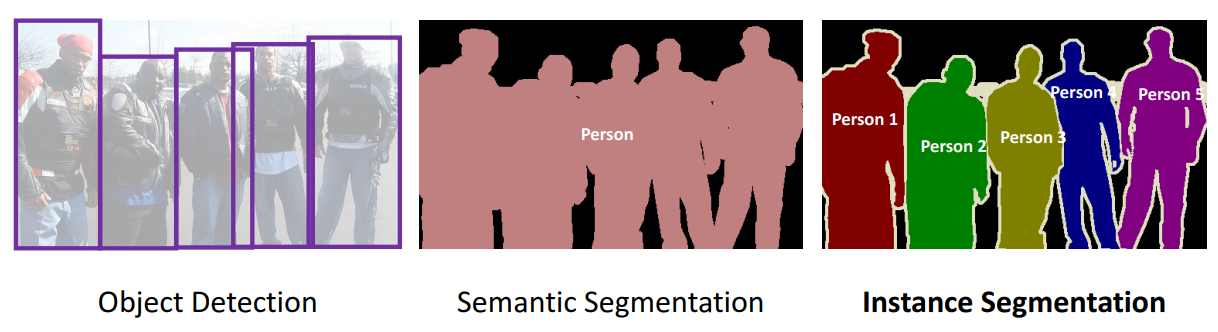
\includegraphics[width=1\textwidth]{yolact} 
    \caption{Difference between object detection, semantic segmentation and instance segmentation}
\end{figure}

On the other hand, image segmentation is the technique which, during the processing and
analysis of digital images, makes it possible to divide an image into parts or regions, often on the basis of pixel characteristics. This technique was mainly developed
to effectively solve problems and critical issues that require detailed information about the objects in an image. Details that cannot be provided at all by classifying
the entire image or parts of it corresponding to a simple box. An important process This important process only ends when the objects, or rather the regions of interest,
have been identified and we move on to the extraction and analysis of the information obtained.
There are two different types of segmentation, the semantic segmentation based on the type of object present, in which all pixels belonging to a type of object are
classified in the same way and marked with a single pixel colour. In contrast, instance-based segmentation derives from the first but differs in that object detection
is also applied to the elements present in the image and each object is classified and instantiated in its own class with a different label.


\section{Thesis goal}
The aim of this thesis is to apply new methods in the field of deep learning to plant phenotyping and to demonstrate how machine learning can accurately identify plant
phenotypic traits and extrapolate their characteristics in order to quickly and accurately help plant breeders to identify plant phenotypes. identify precisely the
phenotypic traits of plants and extrapolate their characteristics in such a way as to help the farmer, the agronomist or the technician in charge of the plant phenotyping
in a fast and precise way. the farmer, agronomist or technician who will manage the plantation. The state of the art will be analysed and it will be illustrated how the
data collection and comparison of the data was carried out. The state of the art will be analysed and it will be explained how to collect data and compare results:
\begin{itemize}
    \item Analysing the state of the art and performance of neural networks with regard to plant phenotyping;
    \item Choosing which networks perform best, implementing them and training them on existing datasets; 
    \item Recreating a controlled environment where measurements can be tested and extrapolated for verification;
\end{itemize}


\section{Thesis structure}
This thesis is structured in five chapters.

The first, as we have just seen, is an introduction to the problem and the techniques that will be used.

The second chapter describes the main articles related to the problem, their approach with different resolutions and their results.

In the third chapter, we present our solution to the problem, how it should be approached, what are the best neural networks that fit the problem and metrics used
for comparisons. the problem and the metrics used for comparisons.

In the fourth chapter, the datasets are presented. In particular, the datasets used for training the networks are shown, followed by the calculation of the metrics
and the comparison with other state-of-the-art methods. the calculation of the metrics and then the comparison with the other methods seen in the state of the art.
Finally, we show our dataset, how it was acquired and its main characteristics, as well as the experimental results collected both by direct measurement and by the
proposed solution. Finally, the metrics related to our dataset are shown.

In the fifth and final chapter, conclusions and possible future developments are discussed.






	
	% 2° Stato dell'arte
	\chapter{Related Works}
	\label{cap:chapter2}
	% !TEX encoding = UTF-8
% !TEX TS-program = pdflatex
% !TEX root = ../main.tex
% !TEX spellcheck = en-EN

%************************************************

\lipsum[1]

\begin{itemize}
	\item \lipsum[2]
	\item \lipsum[3]
\end{itemize} 

\begin{lemma}
	\lipsum[5]
\end{lemma}
\begin{proof}
	\lipsum[6]
\end{proof}

\begin{lstlisting}[language=C, label=lst:c, caption={Hello world!}]
#include <iostream>

using namespace std;

int main() 
{
	cout << "Hello,World!";
	return 0;
}
\end{lstlisting}
	
	% 3° Descrizione algoritmo
	\chapter{Proposed Solution}
	\label{cap:chapter3}
	% !TEX encoding = UTF-8
% !TEX TS-program = pdflatex
% !TEX root = ../main.tex
% !TEX spellcheck = en-EN

%************************************************



Deep learning is showing very effective and promising results in a number of areas, often surpassing those obtained with the old methods. In this chapter we will show
how we apply deep learning techniques to plant phenotyping, in particular we will show how the network used is adapted to different plants and how it can extrapolate
individual leaves from the images.

\section{Our Method}
Segment each instance of a plant is an hard work, images can have different dimension, and each plant can have different position in an image. For this reason, we decided
to identify each plant separately and then go on to identify each instance. In order to classify each plant, we made use of different technologies and we needed to modify
the datasets at our disposal. To do this we used an online tool called Make Sense, which allowed us to create the position annotations of the boxes for object detection.

\subsection{Object Detection}
For the development of object detection of individual plants we used one of the best known and most powerful neural networks in the field of object detection YOLO
\cite{redmon2016look}. This network, taken in version 5, in contrast to the sliding windows, sees the entire image during training and test time so it implicitly encodes
contextual information about classes as well as their appearance. Inside YOLO the separate components of object detection are unified into a single neural network.
It divides the input image into an $S \times S$ grid. If the center of an object falls into a grid cell, that grid cell is responsible for detecting that object.
Each grid cell predicts B bounding boxes and confidence scores for those boxes. Each of this consists of 5 predictions: x, y, w, h, and confidence. The (x, y)
coordinates represent the center of the box relative to the bounds of the grid cell. The width and height are predicted relative to the whole image. Finally
the confidence prediction represents the IOU between the predicted box and any ground truth box.
\begin{figure}[ht] 
    \centering
    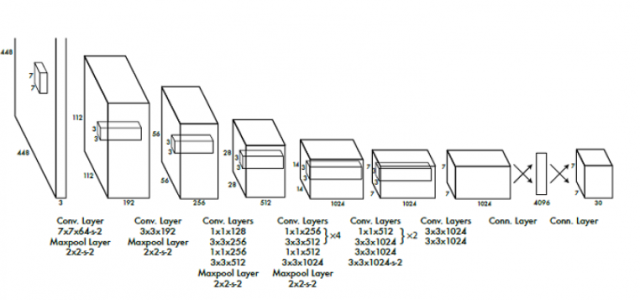
\includegraphics[width=1\textwidth]{yolo_net} 
    \caption{YOLO architecture}
\end{figure}
YOLO is inspired by GoogLeNet \cite{Szegedy_2015_CVPR} model for image classification, it has 24 convolutional layers followed by 2 fully connected layers.
Instead of the inception modules used by GoogLeNet, YOLO simply use $1 \times 1$ reduction layers followed by $3 \times 3$ convolutional layers.

At the end of the training, we used YOLO in such a way as to obtain the individual plants from each image containing different quantities from our dataset. Several
frames are then created, one for each plant identified by the network, which are then placed in a folder and catalogued in two files, one containing the data in COCO
\cite{lin2014microsoft} format, where all the images created are listed, while the second file contains information regarding the position (x, y) in the original image
of the plant just cut out. All this has been created to facilitate the adaptation to the segmentation network and to recompose the data.


\subsection{Instance Segmentation}
The instance segmentation part is performed by BlendMask \cite{chen2020blendmask}. Here we use this convnet in order to segment each instance of leaves. All the leaves found
are saved into a file with the segmentation map still in COCO format. This convnet is a hybrid of top-down and bottom-up approaches, BlendMask consists of a detector
network and a mask branch. The mask branch has three parts, a bottom module to predict the score maps, a top layer to predict the instance
attentions, and a blender module to merge the scores with attentions. 

\begin{figure}[ht]
    \centering
    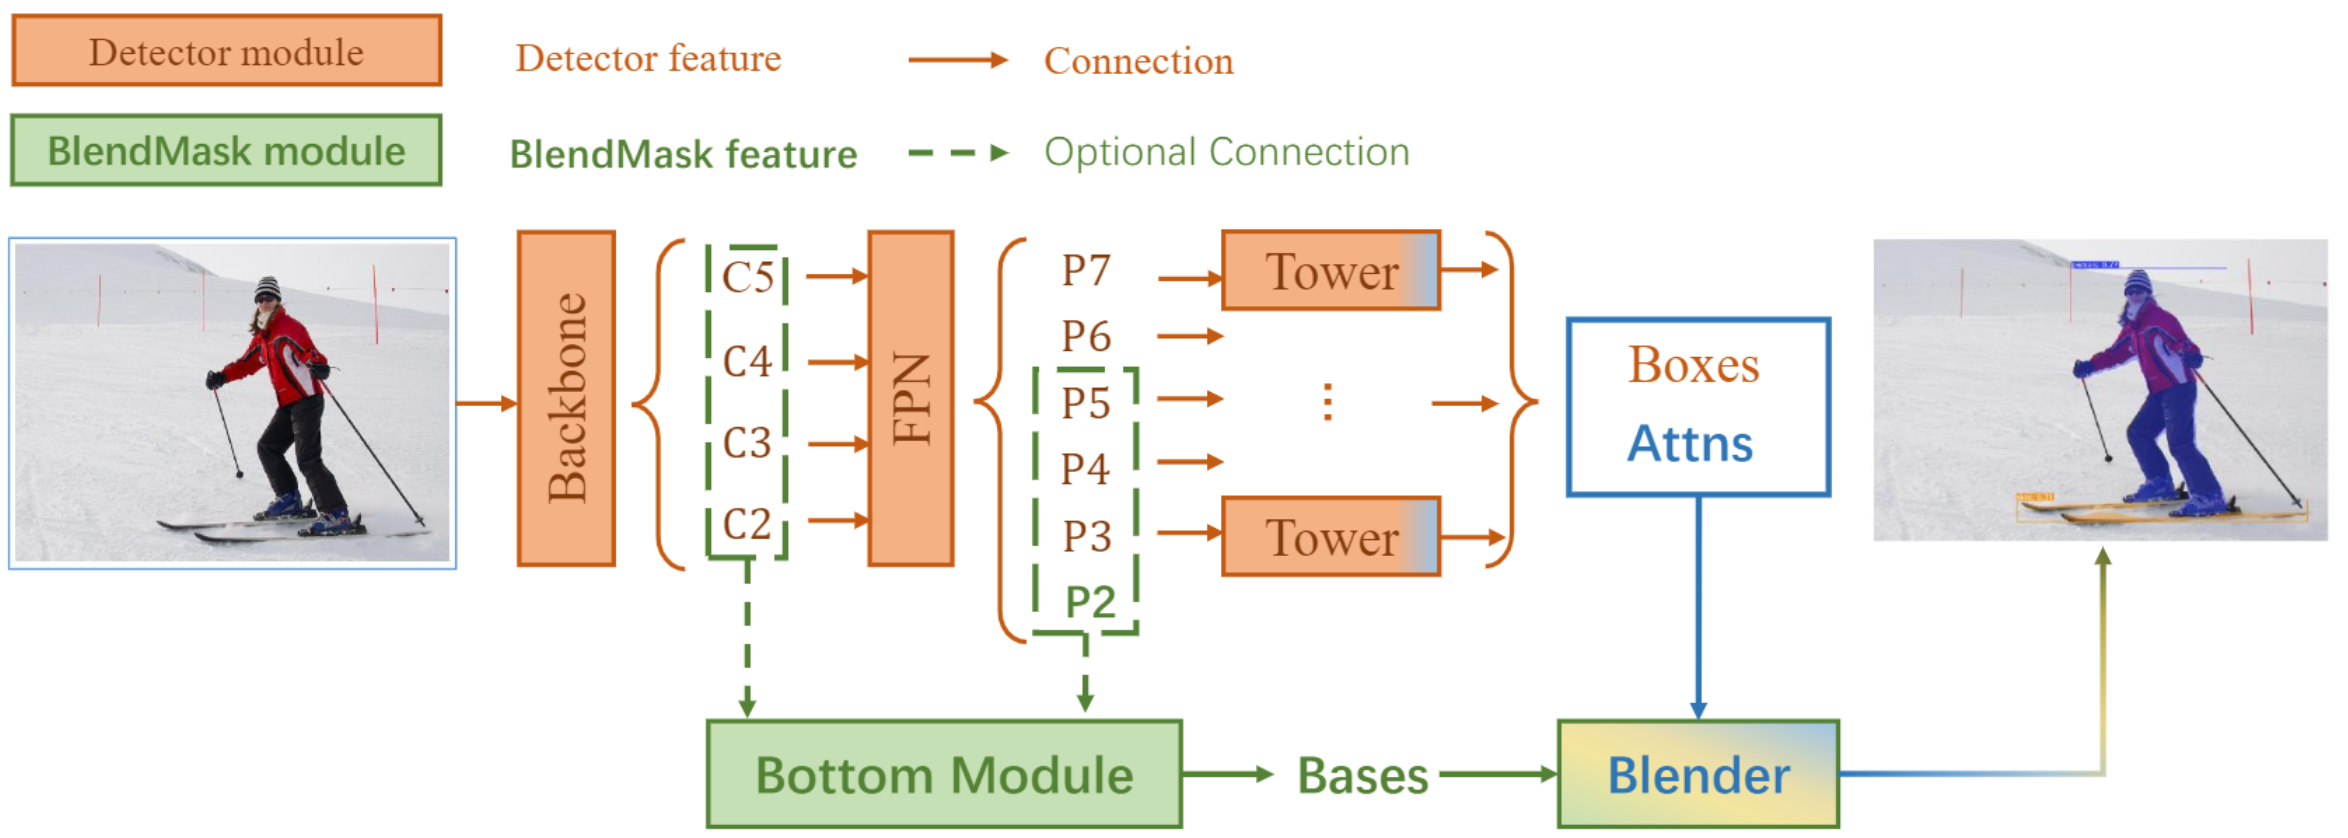
\includegraphics[width=1\textwidth]{blend_net} 
    \caption{Blendmask pipeline overview}
\end{figure}

The bottom module predicting score maps which that are called bases. The input for the bottom module could be backbone features like YOLACT or Panoptic FPN. 
Into the top layer the authors append a single convolution layer on each of the detection towers to predict top-level attentions. Then the blender module get as input the 
bottom-level bases, where with a RoIPooler in Mask R-CNN crops the bases with each proposal, and the it resize the region to a fixed size.
During training, the net simply use ground truth boxes as the proposals. During inference, FCOS \cite{tian2019fcos} predict the results. 

Thanks to this network, we achieved good results in leaf detection and segmentation, so we figured out how to implement the next section that extrapolate the information about
the leaves. 




\subsection{Feature extraction}
After segmentation we collect the information about the extracted leaf and derive only those with a probability of not being covered greater than 80\%.
Next, we save the predictions coming out of the blendmask with the information about both the leaf identifier and the name of the image to which the leaf belongs.
With this, we are able to find out where the leaf is present in the image, so that in the next step we can extrapolate it from the depth image. In this way, we will
finally obtain the 3D image with an rgb part and the fourth dimension, which is the depth. By means of a simple remapping we then obtain the xyz position on the camera plane.
$$
\begin{cases}
    Z = z / depth\_scale \\
    X = (x - cx) * Z / fx \\
    Y = (y - cy) * Z / fy
\end{cases}
$$
Here we have two camera intrinsics which can be used to compute this functions. Those are related to the image which we are refferring to. $cx$, $cy$ are the 
center of camera image while $fx$ and $fy$ are the focal length of the lens. Now with the xyz positions of the image we can finally calculate the various properties. The first
most interesting one will be the area of the leaf for which we will rely on the pyvista \cite{sullivan2019pyvista} library, computed on the mesh surface obtained by the
library itself. This method does not consider the part of the leaf that are overlapped if it is curved, so the surface area could be underestimated. For this reason we
have selected only the leaves which are non overlapped and we have trained the networks with this categories of leaves. Another metrics which we have computed is
the calculation of the major and minor axes, where with scikit-learn \cite{scikit-learn} metrics we have computed the centroids of the leaf and then with the
orientation vector we have computed the length of the axis and the direction. We also calculated the height of the intrinsic leaf with just subtracting the highest
value on the $Z$ axis with the lowest one, and the height of the leaf from the ground, where in a first time we have computed with pyransac3d the plane of the base surface and
then with the points of the leaf we have computed the relative distance from the plane and obtaining the leaf height from the ground.


\section{Used Metrics}
In this section the two evaluation techniques which are used by the referenced paper \cite{scharr2016leaf} the DICE score and the Symmetric Best DICE (SBD).

\subsection{DICE Score}
For semantic and instance segmentation is used the F1 score, or DICE score which is obtained by the fraction of the true positive prediction by the sum of the true positive
with false negative and false positive prediction:
$$F_{1}=\frac{(2)\cdot \mathrm {TP}}{(2)\cdot \mathrm {TP} + 1 \cdot \mathrm {FN} +\mathrm {FP}}$$
which $TP$ are the true positive in the image, $FP$ are the false positive detected pixel and $FN$ are the false negative found in the image.

\subsection{SBD Score}
The other metrics is the Symmetric Best Dice (SBD) \cite{scharr2016leaf}, which is computed by the symmetric average Dice among all objects where for each
input label the ground truth label yielding maximum Dice is used for averaging, to estimate average leaf segmentation accuracy:

\begin{equation}
    BD(L^a, L^b) = \frac{1}{M} \displaystyle\sum_{i=1}^{M} \max_{{1\leq j \leq N}}\frac{2|L_i^a\cap L_j^b|}{|L_i^a|+|L_j^b|}  
\end{equation}

where the $|\cdot|$ is the predicted mask area in pixel and $L_i^a$ for $1\leq i \leq M$ and $L_j^b$ for $i\leq j \leq N$ are sets of leaf
object segments belonging to segmentations of leaves for its corresponding. to subsequently calculate the symmetric, a minimum between
predicted and gt and vice versa must be done:

\begin{equation}
    SBD(L^{ar}, L^{gt}) = \min \{BD(L^{ar}, L^{gt}), BD(L^{gt}, L^{ar})\}
\end{equation}
.



\section{Other Networks}
In order to understand which network was best for our purpose, we used different CNNs, so that we could understand which one was best suited to different types of leaves
in different contexts.


\subsection{YOLACT}
The first network used was YOLACT (You Only Look At CoefficienTs) \cite{bolya2019yolact}. The network proposes to split instance segmentation into two simpler tasks,
first it generates a non-local prototype mask dictionary for the entire image, then it predicts a linear combination of coefficients per instance. Thus, producing
a full-image instance segmentation from these two components is straightforward: for each instance, linearly combine the prototypes using the corresponding
predicted coefficients and then crop with a predicted bounding box. We show that by segmenting in this way, the network learns to locate instance masks on its own,
where visually, spatially and semantically similar instances appear different in the prototype. This approach also has several practical advantages.
First and foremost, it’s fast: because of its parallel structure and extremely lightweight assembly process, YOLACT adds only a marginal amount of computational overhead to
a one-stage backbone detector, making it easy to reach 30 fps even when using ResNet-101. Secondly, the masks are of high quality: since the masks use the full extent of
the image space without any loss of quality from repooling, these masks for large objects turn out to be of significantly higher quality than those of other methods.

YOLACT is composed of different components, the backbone formed by the resnet, is the one used for the classification of the objects present in the scene.
It is flanked by the Feature Pyramid Network (FPN) suitably modified to obtain a more precise classification and, where the softmax cross entropy is used to refine
the prediction process.

\begin{figure}[ht]
    \centering
    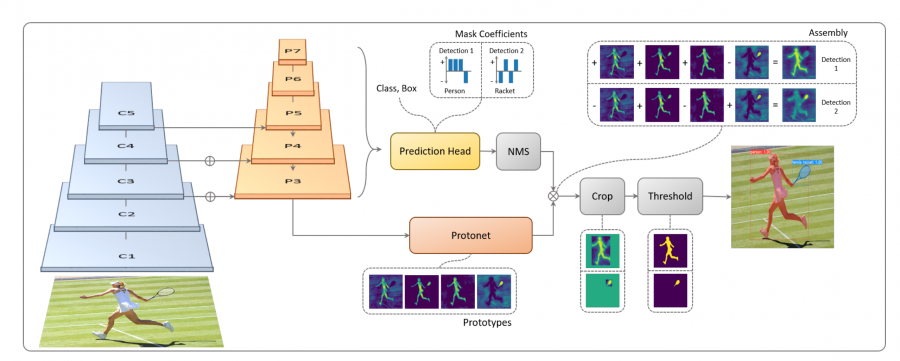
\includegraphics[width=1\textwidth]{yolact_net} 
    \caption{YOLACT model using ResNet-101 + FPN}
\end{figure}

The prototype generation branch (protonet) predicts a set of k prototype masks for the entire image. The authors implemented this protonet as an FCN whose last layer
has k channels and attach it to a backbone feature layer. In addition, taking protonets from the deeper features in the backbone results in more robust masks, and the
higher resolution prototypes produce both higher quality masks and better performance on smaller objects. Thus, we use FPN because its largest feature layers are the deepest.

For mask coefficient prediction, simply the third branch is added in parallel that predicts k mask coefficients, one corresponding to each prototype. Thus, tanh is added
to the k mask coefficients, which produces more stable outputs over no nonlinearity.

Finally mask are recombined, with prototype mask and mask coefficient branch, using a linear combination of the former with the latter as coefficients.

\subsection{YOLACT++}

A similar approach is taken with YOLACT++ \cite{2020}. It is based on the use of the deformed convolutional networks.
Deformable Convolution Networks (DCNs)\cite{dai2017deformable}, \cite{zhu2019deformable} have proven to be effective for object detection, semantic segmentation, and
instance segmentation due to its replacement of the rigid grid sampling used in conventional convnets with free-form sampling.
YOLACT++ was designes following DCNv2, and replace the $3\times 3$ convolution layer in each ResNet block with a $3\times 3$ deformable convolution layer.
Adding deformable convolution layers into the backbone of YOLACT, leads to a +1.8 mask mAP gain. The boost is due to DCN can strengthen the network’s capability of
handling instances with different scales, rotations, and aspect ratios by aligning to the target instances, YOLACT does not have a re-sampling process.
 
\subsection{SOLO}
Instance categories, is the quantized center locations and object sizes, which enables to Segment Objects by LOcations (SOLO) \cite{wang2020solov2}. An image can be
divided into squared number of cells, with the same numbers of center location classes. Each output channel is responsible for one of the central location categories
and the corresponding channel map should predict the instance mask of the object belonging to that location. In essence, an instance position category approximates
the position of the object center of an instance. Thus, classifying each pixel into its instance position category is equivalent to predicting the object center of
each pixel in latent space.

With the SOLO framework, the network optimizes an end-to-end way for the instance segmentation task using mask annotations exclusively, and perform pixel-level
instance segmentation outside the restrictions of local box detection and pixel grouping. For each grid SOLO predicts the C-dimensional output to indicate the
semantic class probabilities, where $C$ is the number of classes. The design is based on the assumption that each cell of the $S\times S$ grid must
belong to one individual instance, thus only belonging to one semantic category.

\begin{figure}[ht]
    \centering
    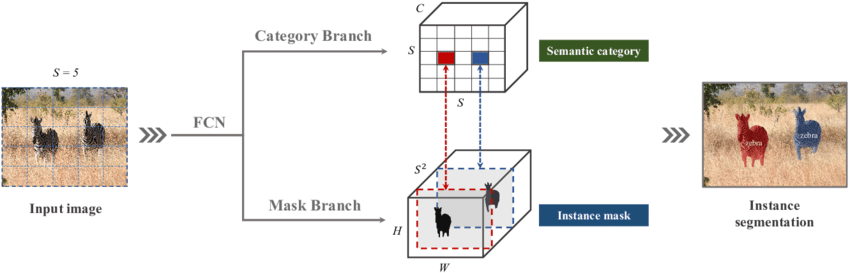
\includegraphics[width=1\textwidth]{solo}
    \caption{SOLO framework, semantic and mask task}
\end{figure}

In parallel with the semantic category prediction, each positive grid cell will also generate the corresponding instance mask. A straightforward approach to
predicting the instance mask is to adopt fully convolutional networks, such as FCNs in semantic segmentation.

SOLO use FPN which generates a pyramid of feature maps with different sizes with a fixed number of channels for each level. These maps are used as input for each prediction
head: semantic category and instance mask.











	
	% 5° Risultati
	\chapter{Experimental Results}
	\label{cap:chapter5}
	% !TEX encoding = UTF-8
% !TEX TS-program = pdflatex
% !TEX root = ../main.tex
% !TEX spellcheck = en-EN

%************************************************
% Parlare dei dataset utilizzati
% parlare di come sono stati raccolti i dati del dataset nostro
% parlare della data augmentation
% parlare dei primi risultati ottenuti
% parlare delle metriche che sono state usate con i corrispettivi risultati


$$
\begin{pmatrix}
    637.735 & 0       & 645.414 \\     
    0       & 637.735 & 349.205 \\
    0       &       0 & 1
\end{pmatrix}
$$


$$
\begin{pmatrix}
    382.641 & 0       & 223.248 \\     
    0       & 382.641 & 233.523 \\
    0       &       0 & 1
\end{pmatrix}
$$
	
	% 6° Conclusione
	\chapter{Conclusion}
	\label{cap:chapter6}
	% !TEX encoding = UTF-8
% !TEX TS-program = pdflatex
% !TEX root = ../main.tex
% !TEX spellcheck = en-EN

%************************************************


The goal of this thesis work was to use neural networks as an alternative to point methods that have been done in the past. So studying the state of the art on the use
of the various solutions developed has allowed us to understand what was the current state of the use of networks in this area.

Subsequently, we studied how neural networks adapted to the different datasets taken into analysis. And finally we analyzed the results obtained comparing them at first
with the reference dataset and then with the komatsuna. The better performances obtained with SOLOv2 also identified a weakness in the network such as the adaptation
to unfamiliar contexts and therefore the difficulty in finding leaf instances.

We can conclude that our method succeeds in dealing effectively with individual plants and that it manages to coincidentally identify both covered and uncovered leaves. 

In the future we can imagine several possible developments both that of an improvement of the networks in order to improve even more the finding of leaf instances but
also that of predictive models able to develop on the basis of the shape and depth images a model able to predict the real size of the leaf, which is difficult at this
time given the visual limitation of still images.





	\blankpage
	
%******************************************************************
% Parte finale
%******************************************************************

	\bibliography{bib} 
	\bibliographystyle{ieeetr}
	
\end{document}